% this file is called up by thesis.tex
% content in this file will be fed into the main document

%: ----------------------- name of chapter  -------------------------
1\chapter{Implementation}\label{implementazione} % top level followed by section, subsection


%: ----------------------- paths to graphics ------------------------

% change according to folder and file names
\graphicspath{{6-implementazione/img/}}


%: ----------------------- contents from here ------------------------
In this chapter we describe our implementation of M2MShare in the ONE simulator, which is described in Chapter \ref{simulatore}. We illustrate some features we added to the simulator, in order to completely emulate M2MShare behaviour and to gather reports data from the simulations we executed.
  

\section{ONE additions}
As we saw in Chapter \ref{m2mshare}, M2MShare is a peer-to-peer protocol which allows the automatic exchange of multimedia content among mobile devices. The ONE is the state-of-the-art regarding movements and connections simulation, especially between mobile nodes, but it has some limitations. Before we could completely implement M2MShare in the simulator, we modified the ONE adding some fundamental features. These allow us to simulate the behaviour of a peer-to-peer protocol with file exchange between network nodes.


\subsection{File Management}
The first step is to add the capability of manage files to nodes. To this purpose, we added a file system to every node, in which to save files to share with other nodes using a P2P application. 
%Node's capabilities are described in class named \textit{DTNHost}


\paragraph{DTNFile}
Every simulated file is an instance of class \textit{DTNFile}, which includes information about the described file:

\begin{itemize}
\item file name
\item file hash value
\item file length, in bytes
\end{itemize}

We do not specify keywords related to that file, which could be useful in implementing a keyword-based search procedure. We did so, because the purpose of our simulations was to emulate and evaluate the behaviour of M2MShare in the second phase of the protocol. In this phase, the user already knows what file it is looking for, so it asks the system to find and download back it, without needing of previous keyword queries. For this purpose a file hash value is sufficient to unambiguously identify the file in the overlay network.


\paragraph{DTNFileSystem}
\textit{DTNFile}s shared by a node are included in an entity called \textit{DTNFileSystem}. As its name suggests, it emulates a mobile device's file system, from an high-level prospective. It has a simple implementation, with a single-level directory structure and functions which allow inserting, deleting and reading files from the file system. To retrieve a file, its hash value is used as search criteria.
\\

The file system presence in a simulated node is optional. For instance, a node emulating a bus do not need a file system. We added new parameters, settable in configuration files, which permit the specification of more options related to file management for a single simulation and increase simulation flexibility: 

\begin{description}
\item[Scenario.simulateFiles] is a boolean parameter that indicates whether or not to simulate the files management in mobile nodes. It applies to the whole simulation.
\item[Group.fileCapability] is a boolean parameter that indicates if nodes belonging to a group can use a file system to store files.
\end{description}

\paragraph{DTNFileGenerator}
\label{fileGeneratorImplementazione}
In a P2P network, shared files are distributed among peers and a user can search between them for the file it is looking for. To emulate the initial files distribution, we implemented a generator which creates and distributes files between nodes at the beginning of the simulation. This generator is initialized using configuration files. Each of them can include several \textit{DTNFileCreationRequest}. These requests describe the files to create and how to distribute them among simulated nodes. During simulation's configuration is possible to set:

\begin{itemize}
\item type of file distribution 
\item name of the \textit{DTNFile}
\item length in bytes
\item number of copies to distribute in the entire network
\end{itemize}

Files are distributed only among nodes which have a file system, that is nodes in groups with \textit{fileCapability} parameter set to \textit{true}. Files distribution can be chosen from the following:

\begin{description}
\item[A] (all): file is distributed among all nodes of the simulation with equal probability
\item[G] (groups): file is only distributed among nodes belonging to specified groups
\item[P] (percent): file is distributed among all nodes of the simulation with probability set in the request
\item[H] (hosts): file is only distributed among specified nodes  
\end{description}

The following are some example of input files used to create and distribute \textit{DTNFiles}, using the \textit{DTNFileGenerator}.

\begin{center}
%\framebox[8cm]{\textbf{A	mySong.mp3	3.5M	50}}
\textbf{A	mySong.mp3	3.5M	50}
\end{center}
Indicates to create a \textit{DTNFile} with size 3,5 MB named "mySong.mp3". The file is copied 50 times and distributed with equal probability among all users with \textit{fileCapability = true}.
\\

\begin{center}
\textbf{P	aPhoto.jpg	5M	25}
\end{center}
Indicates to create a \textit{DTNFile} with size 5.0 MB named "aPhoto.jpg". The file is distributed to 25\% of nodes \textit{fileCapability = true}.
\\

\begin{center}
\textbf{G	aPhoto.jpg	2.4M	25	6	8	10}
\end{center}
Indicates to create a \textit{DTNFile} with size 2,4 MB named "aPhoto.jpg". The file is copied 25 times and distributed with equal probability among all users belonging to groups 6, 8 and 10
\\

\begin{center}
\textbf{H	ebook.pdf	650k	42	43	44}
\end{center}
Indicates to create a \textit{DTNFile} with size 650 kB named "ebook.pdf". The file is distributed among nodes with address 42, 43 e 44, one copy for every node.
\\

We saw in Section \ref{randomness} that an important characteristic of simulations is repeatability. This is fundamental to verify correctness of data and results of completed simulations, or to repeat the simulation changing only few parameters over the total configuration, leaving constant the simulated world description. This applies also to randomness included in \textit{DTNFileGenerator}.\\
To guarantee that repeating one simulation with the same values, same results are achieved, we use a strategy similar to the one adopted by movement models. \textit{DTNFileGenerator} is initialized with a configuration parameter related to \textit{random number generator} seed. If a simulation is repeated several times with the same random seed, files are distributed among the same subset of nodes, at the beginning of the simulation.


%Per garantire che, effettuando più simulazioni utilizzando la medesima configurazione, i files vengano distribuiti agli stessi nodi, è stata adottata la stessa tecnica utilizzata dai modelli di movimento che estendono la classe \textit{MovementModel}. In quel caso i moduli relativi al movimento vengono inizializzati utilizzando un parametro di configurazione relativo al seed per il \textit{random number generator}. Nel caso di valori di configurazione e seed iniziale mantenuti immutati, i nodi si muovono nello stesso modo anche ripetendo più volte la simulazione: vengono infatti generati gli stessi valori relativi a destinazioni, velocità  e tempi di attesa per i nodi.
%\\
%If the seed and all the movement model related settings are kept the same, all nodes should move the same way in different simulations (same destinations, speed and wait time values are used).


\paragraph{FileRequest}
A \textit{FileRequest} represents the user request for a particular file. In every instance of this class are included:
\begin{itemize}
\item \textbf{fromAddr}: the address of the node operated by the user looking for the file
\item \textbf{filename}: the name of the file searched
\item \textbf{creationTime}: the simulated time when the request s submitted by the user 
\end{itemize}
All \textit{FileRequests} are read by the \textit{M2MShareFileRequestReader} at the beginning of every simulation, then during the simulation, when simulated time become equal to the \textit{creationTime} of the \textit{FileRequests}, that is inserted into the correct queue of the node corresponding to the address included in the request.

\paragraph{M2MShareFileRequestReader}
It is the entity responsible for reading the \textit{FileRequests} at the beginning and to dispatch the requests during the simulation, when the correct time comes. It implements the interface \textit{EventQueue}, and so it provides the method \textit{nextEventsTime()}, which returns the instant when the next request will be ready to be inserted in the corresponding node, and the method \textit{nextEvent()}, which returns the next request that will become active.


\subsection{GUI}
The GUI of the ONE simulator has been modified to reflect the addition of file simulation support to the simulator. The detail window related to a node (\figurename~\ref{implRouting-Info}), shown using the button \textquotedblleft Routing info\textquotedblright \ now contains informations about the file system of the node, including all the complete files owned, the number of active tasks and the percent of data already downloaded for each task. 
\begin{figure}[htpb]
  \begin{center}
    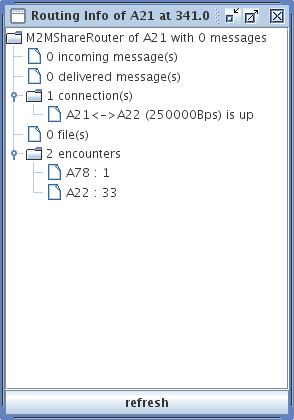
\includegraphics[scale=0.6]{6-implementazione/img/Routing-Info.png}
    \caption{An example of window with a detailed view of a node state}    
    \label{implRouting-Info}
  \end{center}
\end{figure}

\subsection{Reports}
\label{descrReports}
A fundamental feature related to simulations is the ability to gather data from different aspects of the simulated world, like positions of nodes, communications, data transfers and so on. To achieve this goal in the ONE are used some special modules named \textit{Report Generators} which works with some related Listeners to catch the interested events in the simulated scenario and save them to some report files.
The main objectives of our simulations was to gather information about the efficiency of delegations and file division strategies, and to do so we collected data about several aspects for every simulation. We will now describe the report modules created to the gathering of data during the simulations, specifying the type and mode of data collection used.

\paragraph{FileGatheringLog}
The first report module is a log report module, that stores the selected events in a list, saving them to file, one event per line. This module is responsible for listening for the following events:
\begin{itemize}
\item \textbf{VirtualFile creation:} a new \textit{VirtualFile} has been created due to the execution of a \textit{FileRequest} in a node. It emulates a user requesting a new file to be found and downloaded.
\item \textbf{DTNPendingDownload creation:} a new \textit{DTNPendingDownload} has been created in a servant peer thanks to the delegation of a task from a client node.
\item \textbf{DTNPendingDownload completion:} a \textit{DTNPendingDownload} has been completed in a servant peer (the servant has downloaded all the requested file intervals subject of the delegated task). Consequently a \textit{DTNDownloadFWD} has been created and queued in the servant.
\item \textbf{DTNPendingDownload expiration:} a \textit{DTNPendingDownload} has expired in a servant peer before being completed (the servant has not downloaded all the requested file intervals subject of the delegated task).
\item \textbf{DTNDownloadFWD expiration:} a \textit{DTNDownloadFWD} has expired in a servant peer before being completed (the servant has not forwarded all the requested file intervals subject of the delegated task to the requester node).
\item \textbf{DTNDownloadFWD completion:} a \textit{DTNDownloadFWD} has been completed in a servant peer (the servant has forwarded all the requested file intervals subject of the delegated task to the requester node).
\end{itemize}

Every event is saved in the following format:
\begin{center}
\textit{Sim\_time	event\_description	event\_details}
\end{center}
The following are some examples:

\begin{center}
\textbf{15538.0000	PendingDownload	A32 to E476}
\end{center}
Refers to the task delegation from the node A32 to the node E467, 15538 seconds after the beginning of the simulation.
\\

\begin{center}
\textbf{38559.5000 PendingDownload completed in F630 (317200191 requested by A32)}
\end{center}
Refers to the completion of the \textit{DTNPendingDownload} in the servant node F630 at time 38559.5. It was delegated by the node A32 and the id of the searched file was \textit{317200191}
\\

\begin{center}
\textbf{213738.0000	DownloadFWD expired in F523 (317200191 requested by A32)}
\end{center}
Refers to the expiration of the \textit{DownloadFWD} in the servant node F523 at time 213738. It was delegated by the node A32 and the id of the searched file was \textit{317200191}
\\

\paragraph{DataTransferLog}
\textit{DataTransferLog} module is another log module, which keeps track of events regarding data transfer between nodes in the simulation. These can occur during the execution of several activities:
\begin{itemize}
\item \textbf{VirtualFile:} when the requester peer is in range with a node carrying the searched file, and the data transfer take place. Multiple data transfer events can be generated, if there are several peers with the searched file in range.
\item \textbf{DTNPendingDownload:} when a servant peer downloads, from a node carrying the searched file, some requested intervals contained in the delegated task.
\item \textbf{DTNDownloadFWD:} when a servant peer forwards the result of a delegated \textit{DTNPendingDownload} to the client peer.
\end{itemize}
Data transfer events are saved in the following format:
\begin{center}
\textit{Sim\_time	from\_address	to\_address	data\_transferred (in bytes)}
\end{center}
e.g.
\begin{center}
\textbf{98829.0000	G714	A17	2750001}
\end{center}
Refers to the data transfer from node G714 to node A17, 98829 seconds after the start of the simulation. 2750001 bytes have been transferred in this event.
\\

\paragraph{FileGatheringReport}
\textit{FileGatheringReport} module is the most important report module used during our simulations, because it summarizes all key aspects of a single simulation. In detail, these are the values tracked by this module:
\begin{itemize}
\item \textbf{Total data:}	the total amount of data traffic exchanged between servant peers trying to satisfy a delegated task, file possessor peers and the data forwarding quantity toward the requester node.
\item \textbf{VirtualFile created:}	number of \textit{VirtualFile} task created during the simulation
\item \textbf{VirtualFile delegated:} how many times a task has been delegated to a servant peer
\item \textbf{PendingDownloads completed:} how many of the delegated tasks have been completed i.e. how many times the servant peer has been able to locate and download all the data intervals requested in the \textit{DTNPendingDownload} 
\item \textbf{PendingDownloads expired:} how many of the delegated tasks expired before the servant peer being able to find and download all the data intervals requested in the \textit{DTNPendingDownload} 
\item \textbf{DownloadFWDs expired:} how many \textit{DownloadFWDs} expired i.e. the servant peer downloaded all the data intervals requested in the \textit{DTNPendingDownload} but it was not able to forward them to the requester peer before the task expiration
\item \textbf{DownloadFWDs returned:} how many \textit{DownloadFWDs} has been forwarded correctly to the requester peer
\item \textbf{VirtualFile completed:} how many of the created \textit{VirtualFile} has been completed
\item \textbf{First VirtualFile satisfied:}	the time (in seconds) passed from the file request creation before the \textit{VirtualFile} has been completed
\item \textbf{Simulated time:} the simulated duration (in seconds) of the simulation
\item \textbf{Simulation time:}	the real duration of the simulation (in seconds)
\end{itemize}
Saving all these values for every simulation is useful in order to make later analysis such as averages, minimum and maximum values and to find the best or worst case for a large number of simulations.

\paragraph{M2MShareMapCoverageReport}
In order to evaluate the achieved explored area using different delegation strategies we implement the \textit{M2MShareMapCoverageReport}. This module divides the simulated map in squares with size of 10 x 10 meters and counts how many times each square has been visited during the simulation. When a node moves, the module saves its position by adding 1 to the value of the related square. The report is configurable, in order to save only movements related to nodes employing different delegation strategies:
\begin{itemize}
\item the node with the initial file request issued by the user
\item nodes acting as servants, i.e. nodes with delegated tasks received
\item all nodes in the simulation
\end{itemize}
The reason we decided to save all nodes movements, in some simulations, is to obtain a \textit{control set} to evaluate the maximum area that can be explored using certain parameters. By doing so for a high number of simulations we see which parts of the map can be explored (streets, buildings, parks) and which are not (like rivers, the sea or places not reachable with nodes movement).

%
%\paragraph{DelegationGraphvizReport}
%The last report module implemented for our simulation is a module responsible for the creation of reports describing the delegation history of the simulation using a Graphwiz graph. These graphs are described using the DOT language and can be displayed using the \textit{Graphwiz Graph Visualization Software}\footnote{http://www.graphviz.org/}. These graphs are useful to get a visual feedback about the delegations of tasks done and the status of that tasks, especially in case of multi-hop delegations. For every peer involved in delegations can be seen:
%\begin{itemize}
%\item if it receive the delegation (obviously)
%\item if it complete the delegated task
%\item if it forwarded back the result of the delegated task
%\end{itemize}
%In figure \ref{graph-example}
%\figuremacro{graph-example}{Graphviz graph example}{An example of graph generated using the output of DelegationGraphvizReport module}{}


\section{M2MShare Implementation}
In this section we describe the implementation of modules composing M2MShare into the ONE simulator. As said earlier in Section \ref{simulatore}, every routing protocol is an extension of a common superclass named \textit{MessageRouter} and, according to the the ONE philosophy, a new routing module can be inserted extending that class and it can be consequently used in configuration time to set the routing behaviour of nodes.
\\

M2MShare implementation consists in the main class extending \textit{MessageRouter}, named \textit{M2MShareRouter}, and several other classes contained in the package \textit{routing.m2mShare}.

\paragraph{M2MShareRouter}
As mentioned earlier, this is the main class of M2MShare implementation. Its first responsibility is to load the related settings as set in configuration files (see Section \ref{configurazioneONE}) and to initialize all the modules needed for the execution of the protocol. These entities will be described later and are responsible of the different aspects of the protocol. Values used to initialize the settings are read from configuration files and all are included in the settings namespace \textit{M2MShareRouter}. Every parameter has a default value, used in case nothing is not specified in any configuration file. Here the available parameters are shown and, shown in brackets, the relative default value:
\begin{itemize}
\item \textbf{M2MShareRouter.frequencyThreshold [2]} indicates the minimum number of encounters needed to elect a peer as servant and consequently delegate a task to it 
\item \textbf{M2MShareRouter.scanFrequency [10]} indicates how many seconds the \textit{PresenceCollector} must to wait between one scan and the next
\item \textbf{M2MShareRouter.delegationType [1]} indicates the type of delegation strategy used. It accepts three values:
\begin{itemize}
\item \textbf{0:} do not use delegation and file exchange is initiated only when a peer holding the requested data file is found in the reach area 
\item \textbf{1:} use the M2MShare technique where unaccomplished tasks are delegated only to peers which exceed the \textit{frequencyThreshold} value
\item \textbf{2:} use the trivial technique where unaccomplished tasks are delegated to each encountered peer
\end{itemize}
\item \textbf{M2MShareRouter.fileDivisionType [1]} indicates the type of file division strategy used. It accepts three values:
\begin{itemize}
\item \textbf{0:} for every file transfer is requested the entire file
\item \textbf{1:} use the M2MShare technique to choose the initial download point in the requested file
\item \textbf{2:} randomly choose the initial download point in the requested file
\end{itemize}
\item \textbf{M2MShareRouter.useBroadcastModule [true]} used to enable/disable the broadcast module. Could be useful to speed-up simulations, at the cost of a loss of precision
\item \textbf{M2MShareRouter.delegationDepth [1]} indicates the maximum number of delegation hops can be used for delegations, starting from the initial requester
\item \textbf{M2MShareRouter.stopOnFirstFileRequestSatisfied [false]} used to make the simulation stop when the first File Request has been satisfied. Can be useful in simulations in which we are not interested in what happens after the File Request is satisfied
\end{itemize}

%The class \textit{M2MShareRouter} also extends the superclass \textit{MessageRouter} and doing so it override the main method of this class: \textit{update()}. As said in Section \ref{esecuzioneONE}, that method is called one time for every simulated time interval, after the update of movement and connections of the node. In \textit{M2MShareRouter} the only action executed in \textit{update()} is to call the method \textit{runUpdate()} in module \textit{Scheduler}, described in section \ref{schedulerImplementazione}.

\paragraph{PresenceCollector}
The module \textit{PresenceCollector} is responsible for gathering information about in-reach area devices and to track encounters between other nodes to realize the election strategy selected for the current node in the simulation. Encounters data is gathered scanning for in-reach devices with a fixed frequency. When another node exceeds a value named \textit{Frequency Threshold}, it can be elected as a servant and receive unaccomplished tasks as delegations from the current node. Encounters data is saved in a structure called \textit{Servant List} which uses a replacement policy to manage peer slots in the list. If a peer has been encountered for a period greater than a value, called \textit{Probation Window}, without being elected as servant, its slot is freed to give other peers the opportunity to be elected as servants. \textit{PresenceCollector} also includes a tuning algorithm which adapts \textit{Frequency Threshold} and \textit{Probation Window} values at the beginning of every simulated day, according to what observed during the previous day.


\paragraph{Activities}
A single node in M2MShare system can execute several kinds of tasks. In our implementation, each of them is an implementation of interface \textit{DTNActivity} and characterizes one task type respect to another for what concerns their execution. 
\\

In a \textit{VirtualFile} task type, the execution is focused on searching in-reach devices for the file the user asks to find and download. A VirtualFile includes an IntervalMap used to store those file pieces that are still missing. When a VirtualFile task is completed, a new DTNFile is created and saved in the node's file system. 
\\

A VirtualFile can be delegated to a servant peer. When a servant node receives a delegated task, it creates and queues a \textit{DTNPendingDownload} activity. In its execution, the servant node searches in-reach devices for requested intervals of the file described in the delegated task. When a DTNPendingDownload task is completed, the servant node creates end schedules a \textit{DTNForward} task for execution.
\\

In this task's execution, the servant node looks for the client node that delegated it the VirtualFile task. When this node is found, the servant node notifies that it is ready to forward the output of the DTNPendingDownload task. The client can request all or only a subset of intervals the servant downloaded.
\\

Tasks active in servant nodes (DTNPendingDownload and DTNForward) have a TTL value, calculated using client's Probation Window value. When this value is exceeded, the task is deleted from queues and never again scheduled for execution.
\\

With our addition to M2MShare first version, a task can be delegated with more than one hop. To do so we allow M2MShareRouter to delegate also incomplete DTNPendingDownload activities. The result of this delegation, in servant peer, is the creation of a new DTNPendingDownload task. A delegation history list is included in every delegated task. When this second-level task is completed, a new DTNForward task is created in the servant peer. Its execution consists in returning the output of the second-level delegation to one of the nodes in delegation history list. This allows to return the output to the initial requester node faster than returning it following the inverse order of delegation history list.
\\

To avoid generating an high number of delegations, we set a trial period before a servant node delegate again a pending task. It waits one day and during this period it tries to complete the task by itself. If the task is still incomplete after one day, the node proceeds to delegate it for another hop. The maximum number of hops for each delegation is configurable for every simulation. To avoid delegation cycles, we implemented an anti-cycle system similar to the one used in AODV \cite{aodv} which prevents delegating a task to a node that is already acting as servant for it. 

\paragraph{File Division Strategies}
To evaluate the efficiency of M2MShare file division strategy, we implemented a \textit{IntervalMap} according to the one described in Section \ref{descrFileDivisionStrategy}. This structure includes not yet downloaded intervals for a file and is used by our system's Activities to implement the adopted file division strategy. Its behaviour can be set through configuration files for every simulation. This allow emulations of different file division strategies and comparing their efficiency in several simulations:
\begin{itemize}
\item \textbf{M2MShare:} the strategy with dynamic starting point, described in Section \ref{descrFileDivisionStrategy}
\item \textbf{iM:} where each file transfer starts from the beginning of the file
\item \textbf{rM:} where each file transfer starts from a random point within the file
\end{itemize}


\paragraph{Data Transfer}
To emulate data transfers between nodes in the simulated network, we implement a entity named \textit{Communicator}. This entity is used by Activities to emulate the downloading of pieces of files from a file possessor, or the forwarding of a pending task's result to a client node. There is no 1-1 relation between Communicators and Activities. A task can use more than one Communicator when try to simultaneously download pieces of the same file from different sources within communication range. Communicator behaviour is related to the adopted file division strategy, as it influences the starting point of file transfers. Using Communicators allows us to emulate data transfers only when a connection between two nodes is available and to notify information about transfers to related report modules.

%\paragraph{Scheduler}
%\label{schedulerImplementazione}
%\paragraph{Executor}
%\paragraph{Communicator}
%
%\paragraph{BroadcastModule}
 
\section{Analysis}
To evaluate M2Mshare efficiency we need to analyse its performance compared with other strategies or with different versions of M2MShare, as in multi-hop simulations. To do so we repeat each simulation several times changing the random module generators seeds. We do so to achieve results independent from nodes movement and the starting point. For each simulation we save some report files, generated using report modules described in Section \ref{descrReports}. Several analyses have been made over these reports using a set of classes we implemented for this purpose. 
\\

Repeating each simulation with different strategies we are able to compare their performance related to several values. Using our report and analysis modules, for each single simulation we are able to evaluate:
\begin{itemize}
\item number of File Requests created
\item how many tasks have been delegated during the simulation
\item how many delegated tasks have been completed
\item how many delegated tasks expired before completion
\item how many delegated tasks have been completed but expired before the result was forwarded to the requester node
\item number of File Request satisfied
\item after how much time a File Request has been satisfied
\item the length of simulated time
\item the length of the simulation (in real time)
\end{itemize} 

For each set of simulations repeated changing random generators seeds, we are able to evaluate 
\begin{itemize}
\item minimum value
\item maximum value
\item average value
\end{itemize} 
related to each of the parameters above.
 
% ---------------------------------------------------------------------------
%: ----------------------- end of thesis sub-document ------------------------
% ---------------------------------------------------------------------------

